% !TeX root = ./main.tex
% chktex-file 46
% !TeX spellcheck = en-GB
% !TeX encoding = utf8

% ****** Start of file apssamp.tex ******
%
%   This file is part of the APS files in the REVTeX 4.1 distribution.
%   Version 4.1r of REVTeX, August 2010
%
%   Copyright (c) 2009, 2010 The American Physical Society.
%
%   See the REVTeX 4 README file for restrictions and more information.
%
% TeX'ing this file requires that you have AMS-LaTeX 2.0 installed
% as well as the rest of the prerequisites for REVTeX 4.1
%
% See the REVTeX 4 README file
% It also requires running BibTeX. The commands are as follows:
%
%  1)  latex apssamp.tex
%  2)  bibtex apssamp
%  3)  latex apssamp.tex
%  4)  latex apssamp.tex
%
\documentclass[%
 reprint,
%superscriptaddress,
%groupedaddress,
%unsortedaddress,
%runinaddress,
%frontmatterverbose, 
%preprint,
%showpacs,preprintnumbers,
%nofootinbib,
%nobibnotes,
%bibnotes,
 amsmath,amssymb,showkeys,
 aps,
%pra,
%prb,
%rmp,
%prstab,
%prstper,
%floatfix,
]{revtex4-1}

\usepackage{graphicx}% Include figure files
\usepackage{dcolumn}% Align table columns on decimal point
\usepackage{bm}% bold math
\usepackage{hyperref}% add hypertext capabilities
\usepackage{todonotes}
\usepackage{float}
\usepackage{mathtools}
\usepackage{csquotes}
\usepackage{cleveref}
\usepackage{braket}


\DeclarePairedDelimiter\abs{\lvert}{\rvert}%
\DeclarePairedDelimiter\norm{\lVert}{\rVert}%

\begin{document}

\title{Corona Contact Tracing:\\Optimal contact inhibition for decelerating the pandemic}

\author{Leonard Salewski}
\author{Thomas Hoffmann}
\author{Matthias Blaschke}
\author{Martin Lellep}

\date{03/22/2020}

\begin{abstract}
	
	\begin{description}
		\item[Scope] Created during the \#WirVSVirus Hackathon of the German government as initiative\\against the spreading of the COVID-19 pandemic in early 2020.
		\item[Open source] Available under \url{https://github.com/PellelNitram/corona_contact_tracing}.
	\end{description}

	% \todo[inline]{Finalise abstract as last part.}
	
	In this work we develop a graph convolutional approach to predict the health status of all agents in this simulation.	It uses past contacts as well as observed health information to derive this prediction.
	It is able to deal with partial data such as missing locations and missing health status, as it is a probabilistic approach.
	
	Lastly, this prediction can be used to derive measures to reduce the diseases' spread.
	We propose to find a optimal trade of between removing the least amount of edges in said graph (e.g.\ through quarantine, social distancing, etc.) and limiting the spread of the disease.
	% Such trade of could be found with minimal cut algorithms.
	Opposed to classical non-pharmaceutical intervention methods such as contact tracing, our approach directly identifies the nodes with the greatest potential to accelerate the diseases' spread in the network.
	
	This technical report was created within the \#WirVsVirus Hackathon of the German government and is Work in Progress!

\end{abstract}

\keywords{SARS-COV-19, COVID-19, Graph Convolution}

\maketitle

\section{\label{sec:introcution}Introduction}

% !TeX root = ./main.tex
% chktex-file 46
% !TeX spellcheck = en-GB
% !TeX encoding = utf8

The outbreak of the SARS-COV-2 virus and the associated COVID-19 illness sweep rapidly across the world. Some patients need ventilation support to survive and the exponential growth in infected persons quickly overwhelms any available medical resources~\cite{10.1001/jama.2020.2648}.

Thus the identification of contact persons is of great importance to control the spread of the disease. Some governments, such as the Singapurian, use location trace data from mobile phone providers. Other approaches are more user centric and build apps that utilise GPS data of individuals.

It is known from past outbreaks and epidemiologic research that such contact tracing and non pharmaceutical interventions (NPI) like school cancellations are important tools to reduce the impact of crisis like the ongoing one. However, both are not particularly directed interventions might come at the cost of an increased social or economic cost.

We formulate a mathematical framework that is suitable to be used for subsequent optimisations which contacts should be avoided while on the other hand decreasing the social and economic cost.

The section~\ref{sec:basics} will explain the mathematical foundations that are necessary to understand our main approach presented in section~\ref{sec:framework}. Sections~\ref{sec:working_state} and~\ref{sec:outlook} present our working state at the end of the \#WirVsVirus hackathon and provide extensive outlook, respectively. In the outlooks, additionally, we propose to use mathematical optimisation to compute very targeted NPIs (e.g.\ only cancellation of large events) and optimal placement of limited tests (e.g.\ prioritize potential super spreaders). These perspectives have the potential to control the disease with minimal effects on daily life.

\section{\label{sec:basics}Mathematical basics}

\subsection{Graphs and graph convolutions}

Graphs are sets of nodes connected by edges, as shown in Fig.~\ref{fig:graph_example}

\begin{figure}[H]
	\centering
	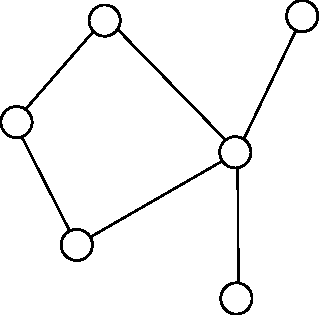
\includegraphics[width=0.4\columnwidth]{img/graph_example.pdf}
	\caption{Example graph.}
	\label{fig:graph_example}
\end{figure}

We model partially infected populations as a graph, where each individual (interchangeably called agent) is a node. Edges of this graph model contacts between two agents. The dynamics of infections throughout the population is described by graph convolutions. The definition of a graph convolution~\cite{Kipf2017SemiSupervisedCW} for here is

\begin{equation}
	\label{eq:graph_convolution}
	h_{v_i}^{(l+1)} = \sum_{j\in A(i)} h_{v_j}^{(l)}
\end{equation}

with $h_{v_i}^{(l)}$ denoting the feature vector of node $i$ of iteration $(l)$ and $A(i)$ as all neighbours of node $i$ as described by the adjacency matrix $A$. This formulation is equivalent to the matrix formulation $h^{(l+1)} = A h^{(l)}$ with $A$ as adjacency matrix as shown in \ref{sec:consistency}. We consider here adjacency matrices without diagonal elements.

Each agent $i$ is modeled by $D$ features, $h_{v_i} \in \mathbb{R}^D$. Therefore, the feature matrix, $h^{(l)}$, consists of all agents' features at time $(l)$ and is thereby of dimension $N\times D$ where there are $N$ agents in the population and each agent is described by $D$ features. A three dimensional feature space is used in this work, $D=3$, modeling three possible health states. The unit vectors of this space are interpreted as following:
\begin{itemize}
	\item $\vec{e}_0$: susceptible state
	\item $\vec{e}_1$: infected state
	\item $\vec{e}_2$: recovered state
\end{itemize}
A uniform distribution over these possible states expresses complete uncertainty of the health state of an agent.

\subsection{SIR Model}

Our basic stochastic SIR model relies on the assumptions that every person in an environment can be modeled as a point value, which has a location (i.e.\ GPS coordinates) and an infection state. These states can be either \textit{susceptible} (S), \textit{infected} (I), \textit{recovered} (R) or in advanced models also \textit{under quarantine} (Q) or \textit{dead} (D). All individuals, here called agents, have a probability (here called diffusion rate $d$ to make a step per time step on a predefined grid. In the case, that some agents meet at the same location, disease spreading can occur. An infected agent spreads the disease with probability $\beta$ to all the agents in its close vicinity (same location on the grid). Furthermore recovery is covered by taking a recovery rate into account, i.e.\ a probability $\gamma$ to recover from the disease per time step. If an infected agent recovers from the disease, the state of the agent changes from \textit{infected} to \textit{recovered}, which is definite (no double infections). The process ends, when no infected agents are left.
\begin{center}
	Susceptibles $\overset{\beta}{\longrightarrow}$ Infected $\overset{\gamma}{\longrightarrow}$ Recovered.
\end{center}

An example of a early model state is shown in Figure~\ref{fig:1}

\begin{figure}[H]
	\centering
	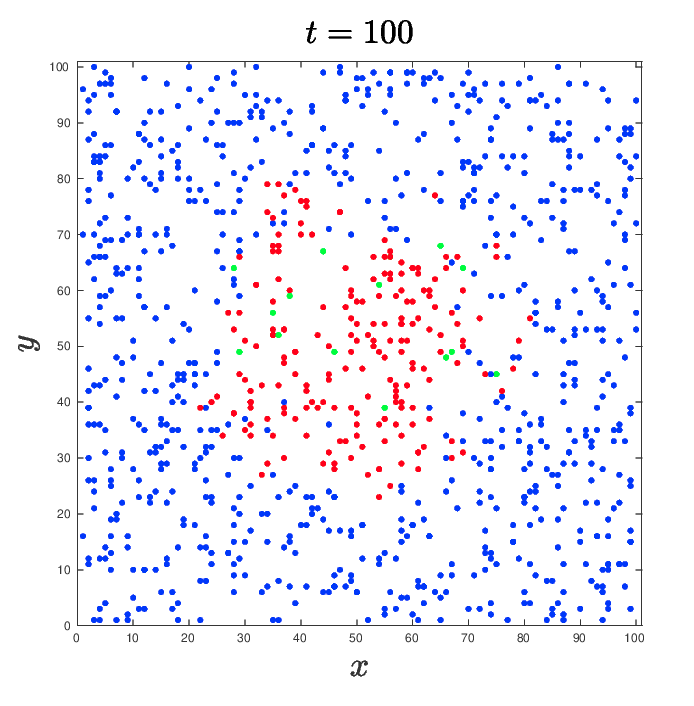
\includegraphics[width=0.4\linewidth]{initial_setup.png}
	\caption{Early state of SIR model, blue dots = susceptibles, red dots = infected agents, green dots = Recovered agents}%
	\label{fig:1}
\end{figure}

In this case, 1000 agents were initialized on a 100 by 100 grid, where a certain amount of infected agents were introduced as a seed. Letting the agents perform random walks on the grid (maximally one step each time step with probability $d$), and letting the model converge, the results in figure~\ref{fig:2} can be observed.

\begin{figure}[H]
	\centering
	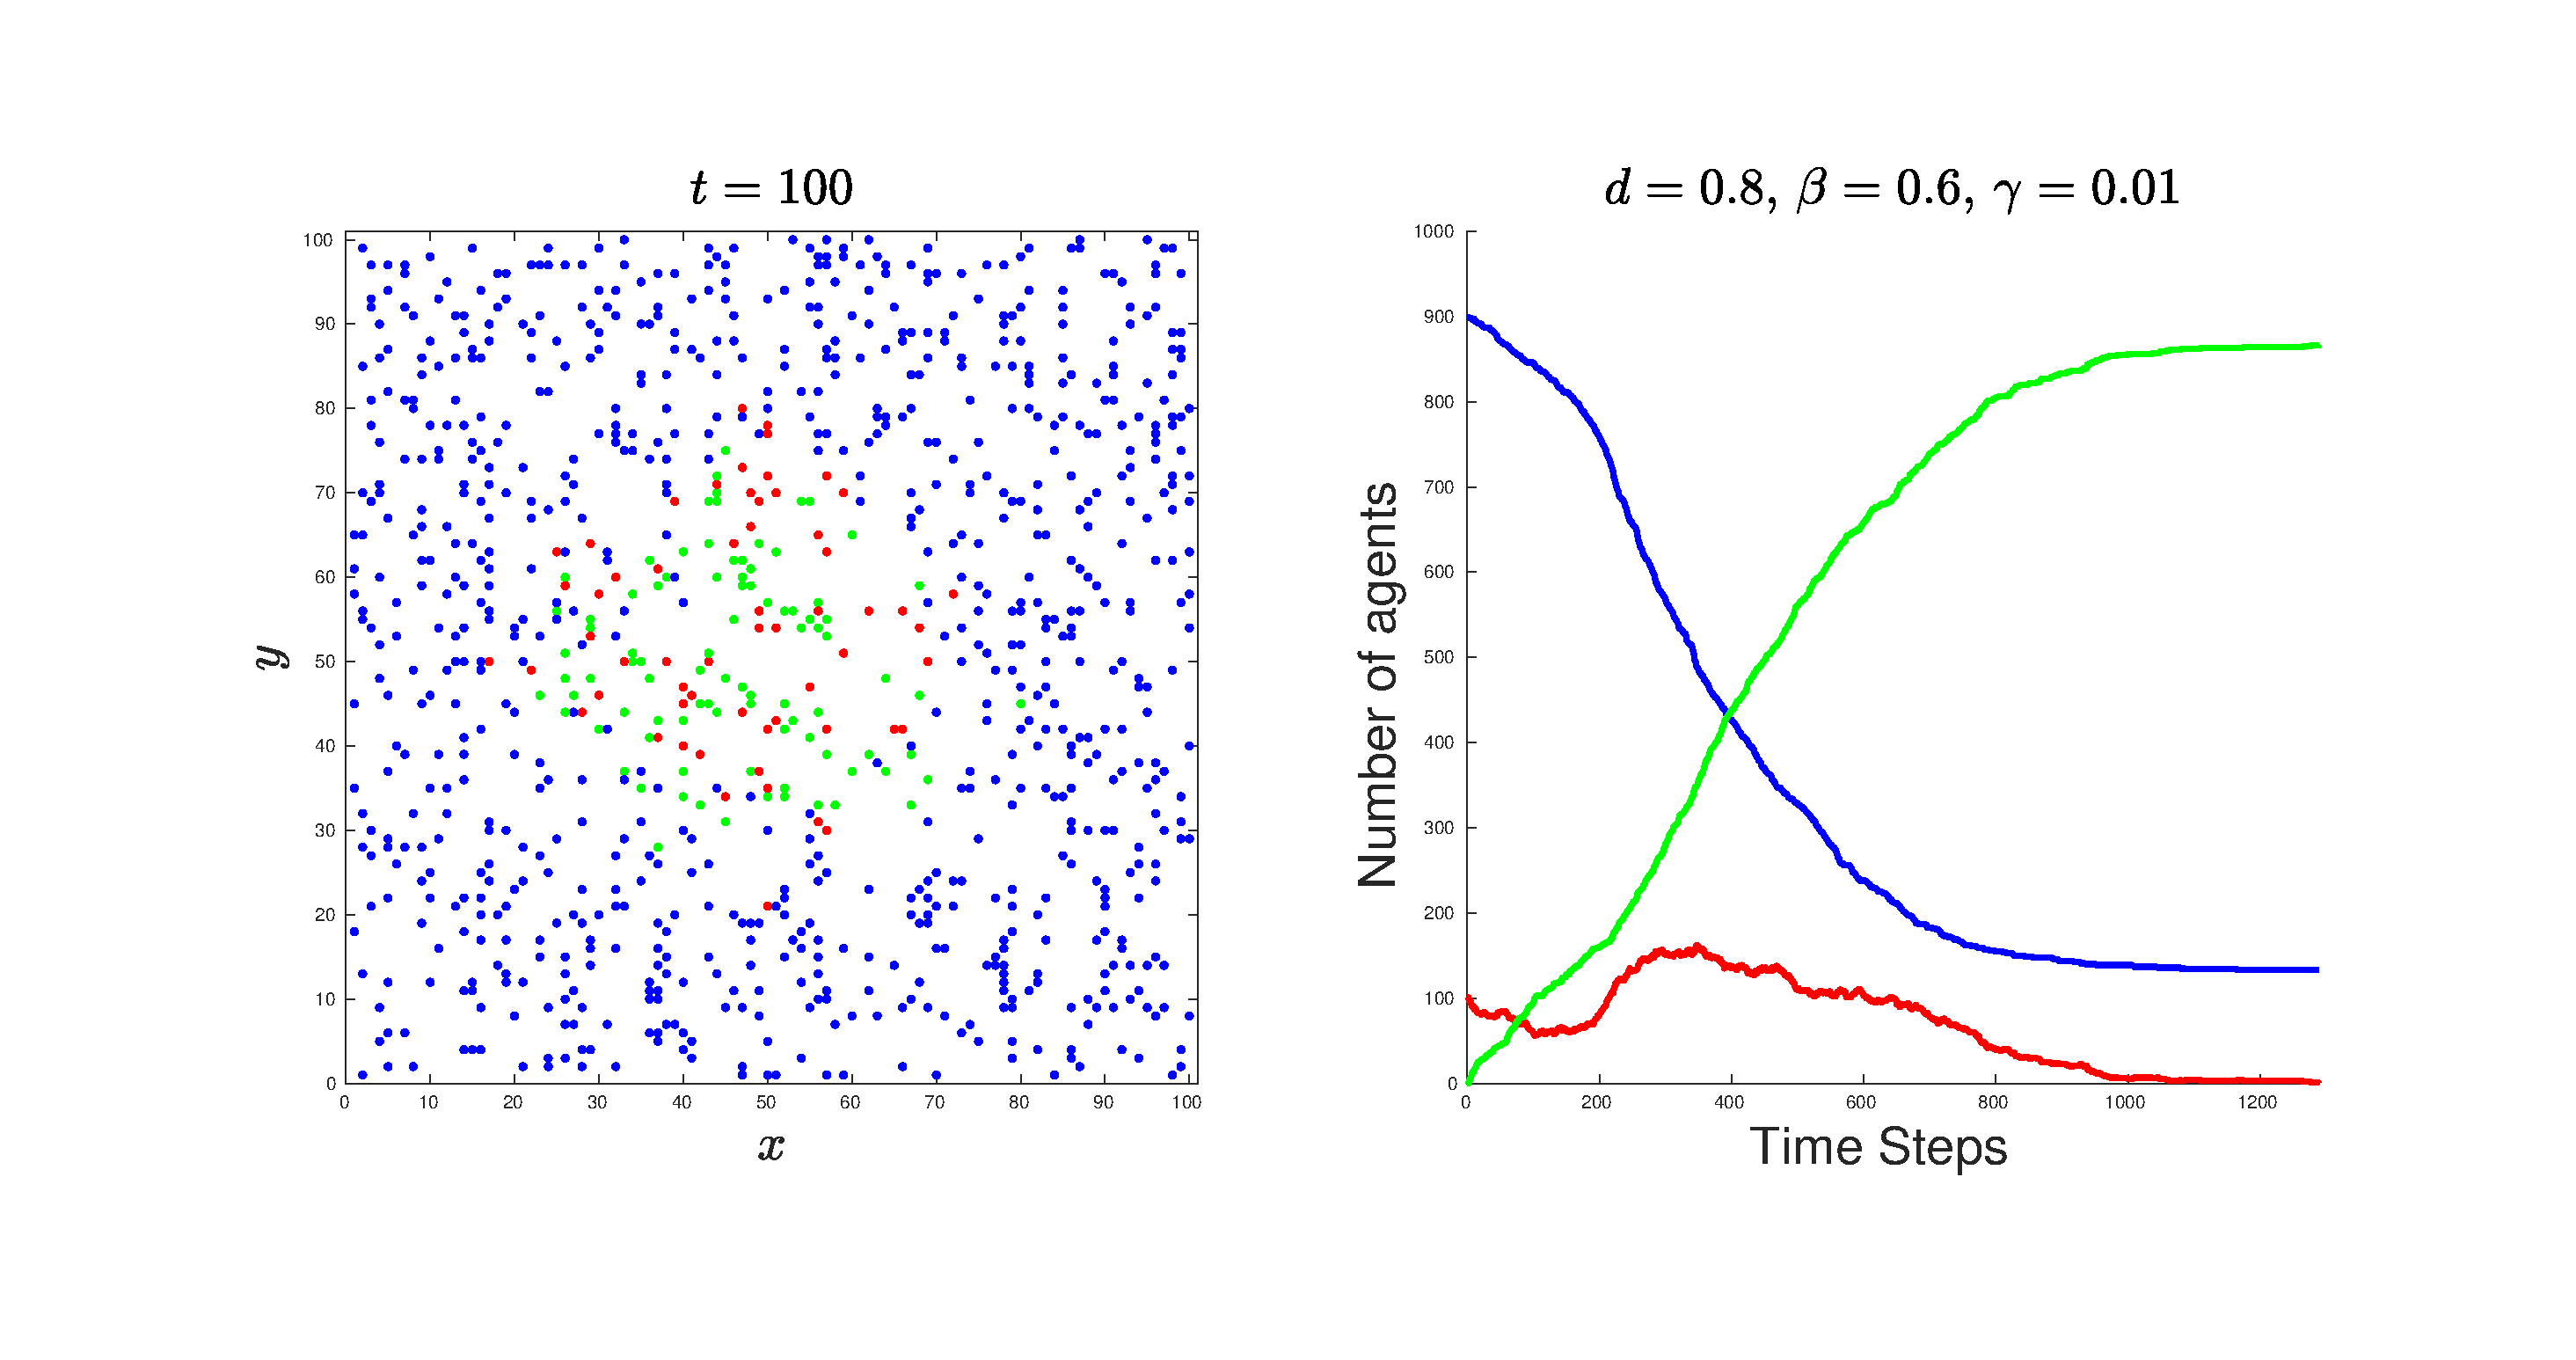
\includegraphics[width=0.9\linewidth]{1_1000_agents}
	\caption{Plot of the proportions of susceptible (blue), infected (red) and recovered (green) individuals in each state over time.}%
	\label{fig:2}
\end{figure}

With the above stated parameters ($d=0.8$, $\beta=0.6$, $\gamma=0.01$), the disease does not spread over the whole population. However over 80\% were infected over time, which could be a very likely scenario of the corona out brake.

\subsection{Improving the Simulation}
Random walk is commonly used for simple Simulations. However this movement pattern does not represent the daily routine of the majority of citizens. It  is more likely that the major part of the population moves around their hometown and travel small distances which leads to clustering of the whole population. To improve the simulation the agents are split into two groups. One group moves random walk like. This group represents e.g. service providers and delivery services. The other group moves around given points. This movement is implemented using polar coordinates with random radius and random angle. The movement pattern of the two groups is illustrated in figure \ref{fig:movementPattern}. 
\begin{figure}[H]
	\centering
	\includegraphics[width=0.9\linewidth]{docs/movementPattern.png}
	\caption{Movement pattern of the two groups. Random walk (orange) and localized movement (blue)}%
	\label{fig:movementPattern}
\end{figure}

With these two groups new features like multiple outbreaks of the waves in different clusters can be observed. An example of the improved model is shown in figure \ref{fig:multipleOutbreaks}. The infection waves at $t = 40$, $t = 210$ and $t= 650$ can be explained by the infection of a new cluster.  

\begin{figure}[H]
	\centering
	\includegraphics[width=0.7\linewidth]{docs/multipleOutbreaks.pdf}
	\caption{Plot  of  the  proportions  of  susceptible  (blue),  infected  (orange)  and  recovered  (green)  individuals  in  each  state over time.)}%
	\label{fig:multipleOutbreaks}
\end{figure}

\section{\label{sec:framework}Graph-based framework}

- novel graph-based approach to

- To accurately model the disease, there is graph contribution and an individual health contribution.

\subsubsection{Explanation of the graph contribution term}
The graph contribution models how infected agents spread the disease through contacts with susceptible agents.

\begin{equation}
h_{v_i, m}^{(l+1)}
=
\underbrace{
	\sum_k \textcolor{red}{\frac{\hat{A}_{v_i, k}^{(l)}}{\sum_j \hat{A}_{v_i, j}^{(l)}}} h_{k, m}^{(l)} \textcolor{blue}{\delta_{m, e_I}}
}_{\text{Graph}}
\end{equation}

\begin{itemize}
	\item A sum over all agents' features $h_{k,m}^{(l)}$ is weighted by the normalised infection-adjusted graph connections as shown in red.
	\item The Kronecker delta, as shown in blue, ensures that only the I feature is added as this is the only one that matters during social contacts between agents.
	\item The infection-adjusted adjacency matrix $\hat{A}$ is constructed from $A$ and $I$ which are the regular continuous adjacency matrix and the infection matrix, respectively. These three quantities are explained in the following:
	\begin{itemize}
		\item The adjacency matrix $A$ is time dependent, $A^{(l)}$, and inferred from data. In our use case, $A_{ij} = \frac{1}{dist(v_i, v_j)+\epsilon}$, hence $A_{ij}$ is large when persons $i$ and $j$ have been in contact. $\epsilon$ serves as regularization for small distances.
		\item The infection matrix is constructed as
		\begin{equation}
		I =
		\begin{pmatrix}
		0     &  0  & 0 \\
		\beta &  0  & \alpha \\
		0     &  0  & 0
		\end{pmatrix}
		=
		(I_{ij})_{i,j}
		\end{equation}
		with $i$ as the index of the host state and $j$ is the index of the contact person state. The states that we consider here are ordered as follows: susceptible, infected, recovered. $\beta$ denotes the probability of infection  after contact (also known as attack rate). $\alpha$ models the probability of being reinfected, which we assume to be zero ($\alpha=0$) based upon current medical \todo{cite!}research.
		\item $\hat{A}$, with $\hat{A}_{ij}\in [0, 1]$, is the adjacency matrix that takes the infection interactions into account and is computed as follows
		\begin{equation}
		\hat{A}_{ij} = A_{ij}\cdot \frac{ h_{v_1}^T I h_{v_2} + h_{v_2}^T I h_{v_1} }{\beta}.
		\end{equation}
		The weighted scalar product of the health states of agents $i$ and $j$ is used to evaluate whether the edge is relevant for the infection dynamics. Only when an infected person and a susceptible have contact, the edge $A_{ij}$ should be considered, otherwise it should be dropped.	The sum in the denominator comes from the fact that both, agent $i$ and $j$, can act as host during a contact. The division by $\beta$ normalises the factor to one to ensure $\hat{A}_{ij} \in [0, 1]$. Since $I$ is not symmetric, $p_a$ is a proper normalization because the sum is in $\{0, p_a\}$. Note that the fraction has the desired properties for pure $S$-, $I$- and $R$-persons.
	\end{itemize}
\end{itemize}


\subsubsection{Temporal}
% \item Explanation of the temporal term:
The transition of a persons' health state $h_{v_i}^{(l)}$ is determined by the following assumptions:
\begin{itemize}
	\item A susceptible person always stays susceptible
	\item An infected person has a probability $\gamma$, called recovery rate, to recover. The remaining probability $1-\gamma$ denotes that the person stays sick.
	\item A recovered person could have a probability to be re-infected, but we assume this to be zero. Thus a recovered person always stays recovered.
\end{itemize}
Thus the temporal transition matrix $T$ is:
\begin{equation}
T = 
\begin{pmatrix}
1 &     0    & 0      \\
0 & 1-\gamma & \gamma \\
0 &     0    & 1      \\
\end{pmatrix}
\end{equation}
The temporal update rule based on the health status thus becomes:
\begin{equation}
H^{(l+1)} = H^{(l)} T
\end{equation}

\subsubsection{Joint Model}

Our main propagation rule is based on the definition of a graph convolution shown in Eq.~\eqref{eq:graph_convolution} and reads as follows in component notation
\begin{equation}
h_{v_i, m}^{(l+1)}
=
\underbrace{
	\sum_k \textcolor{red}{\frac{\hat{A}_{v_i, k}^{(l)}}{\sum_j \hat{A}_{v_i, j}^{(l)}}} h_{k, m}^{(l)} \textcolor{blue}{\delta_{m, e_I}}
}_{\text{Graph}}
+
\underbrace{
	{(h_{v_i}^{(l)}\cdot T)}_m
}_{\text{Temporal}}
\end{equation}
with $m$ being the index of the health state.

This propagation rule is based on the following aspects:

\begin{itemize}
	\item The propagation consists of two parts, first the graph contribution and second the temporal contribution. While the former captures the dynamics of infections based on the social contacts between agents, the former ensures that an infected agent heals over time and becomes resistant against the Corona virus.
\end{itemize}

\section{\label{sec:working_state}Current working state}

\subsection{SIR Model}

For testing and data generation we have implemented a SIR Model using Python. The code can be found in the given Github repository.\newline
An example of an early model state is shown in Figure~\ref{fig:1}.

\begin{figure}[H]
	\centering
	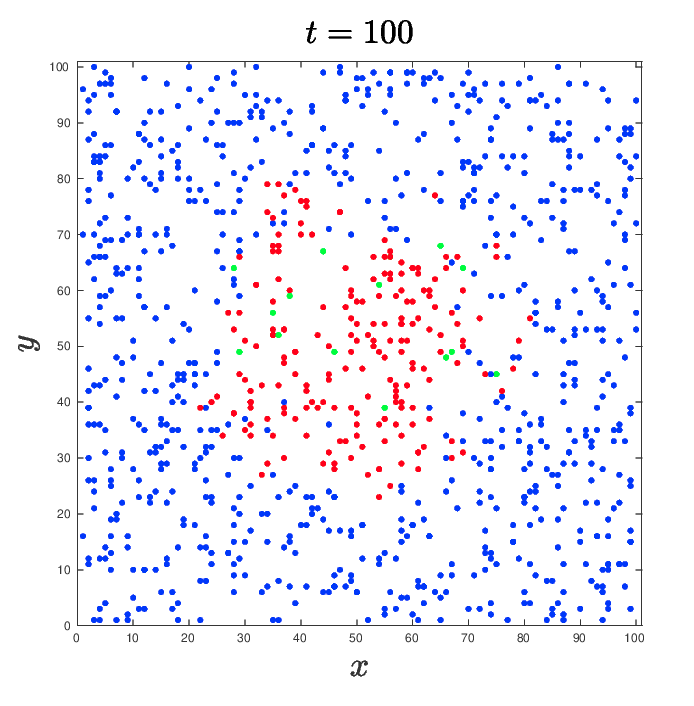
\includegraphics[width=0.4\linewidth]{initial_setup.png}
	\caption{Early state of SIR model, blue dots = susceptibles, red dots = infected agents, green dots = recovered agents.}%
	\label{fig:1}
\end{figure}

In this case, 1000 agents were initialized on a 100 by 100 grid, where a certain amount of infected agents were introduced as a seed. Letting the agents perform random walks on the grid (maximally one step on the grid each time step with probability $d$) and letting the model converge, the results in Figure~\ref{fig:2} can be observed.

\begin{figure}[H]
	\centering
	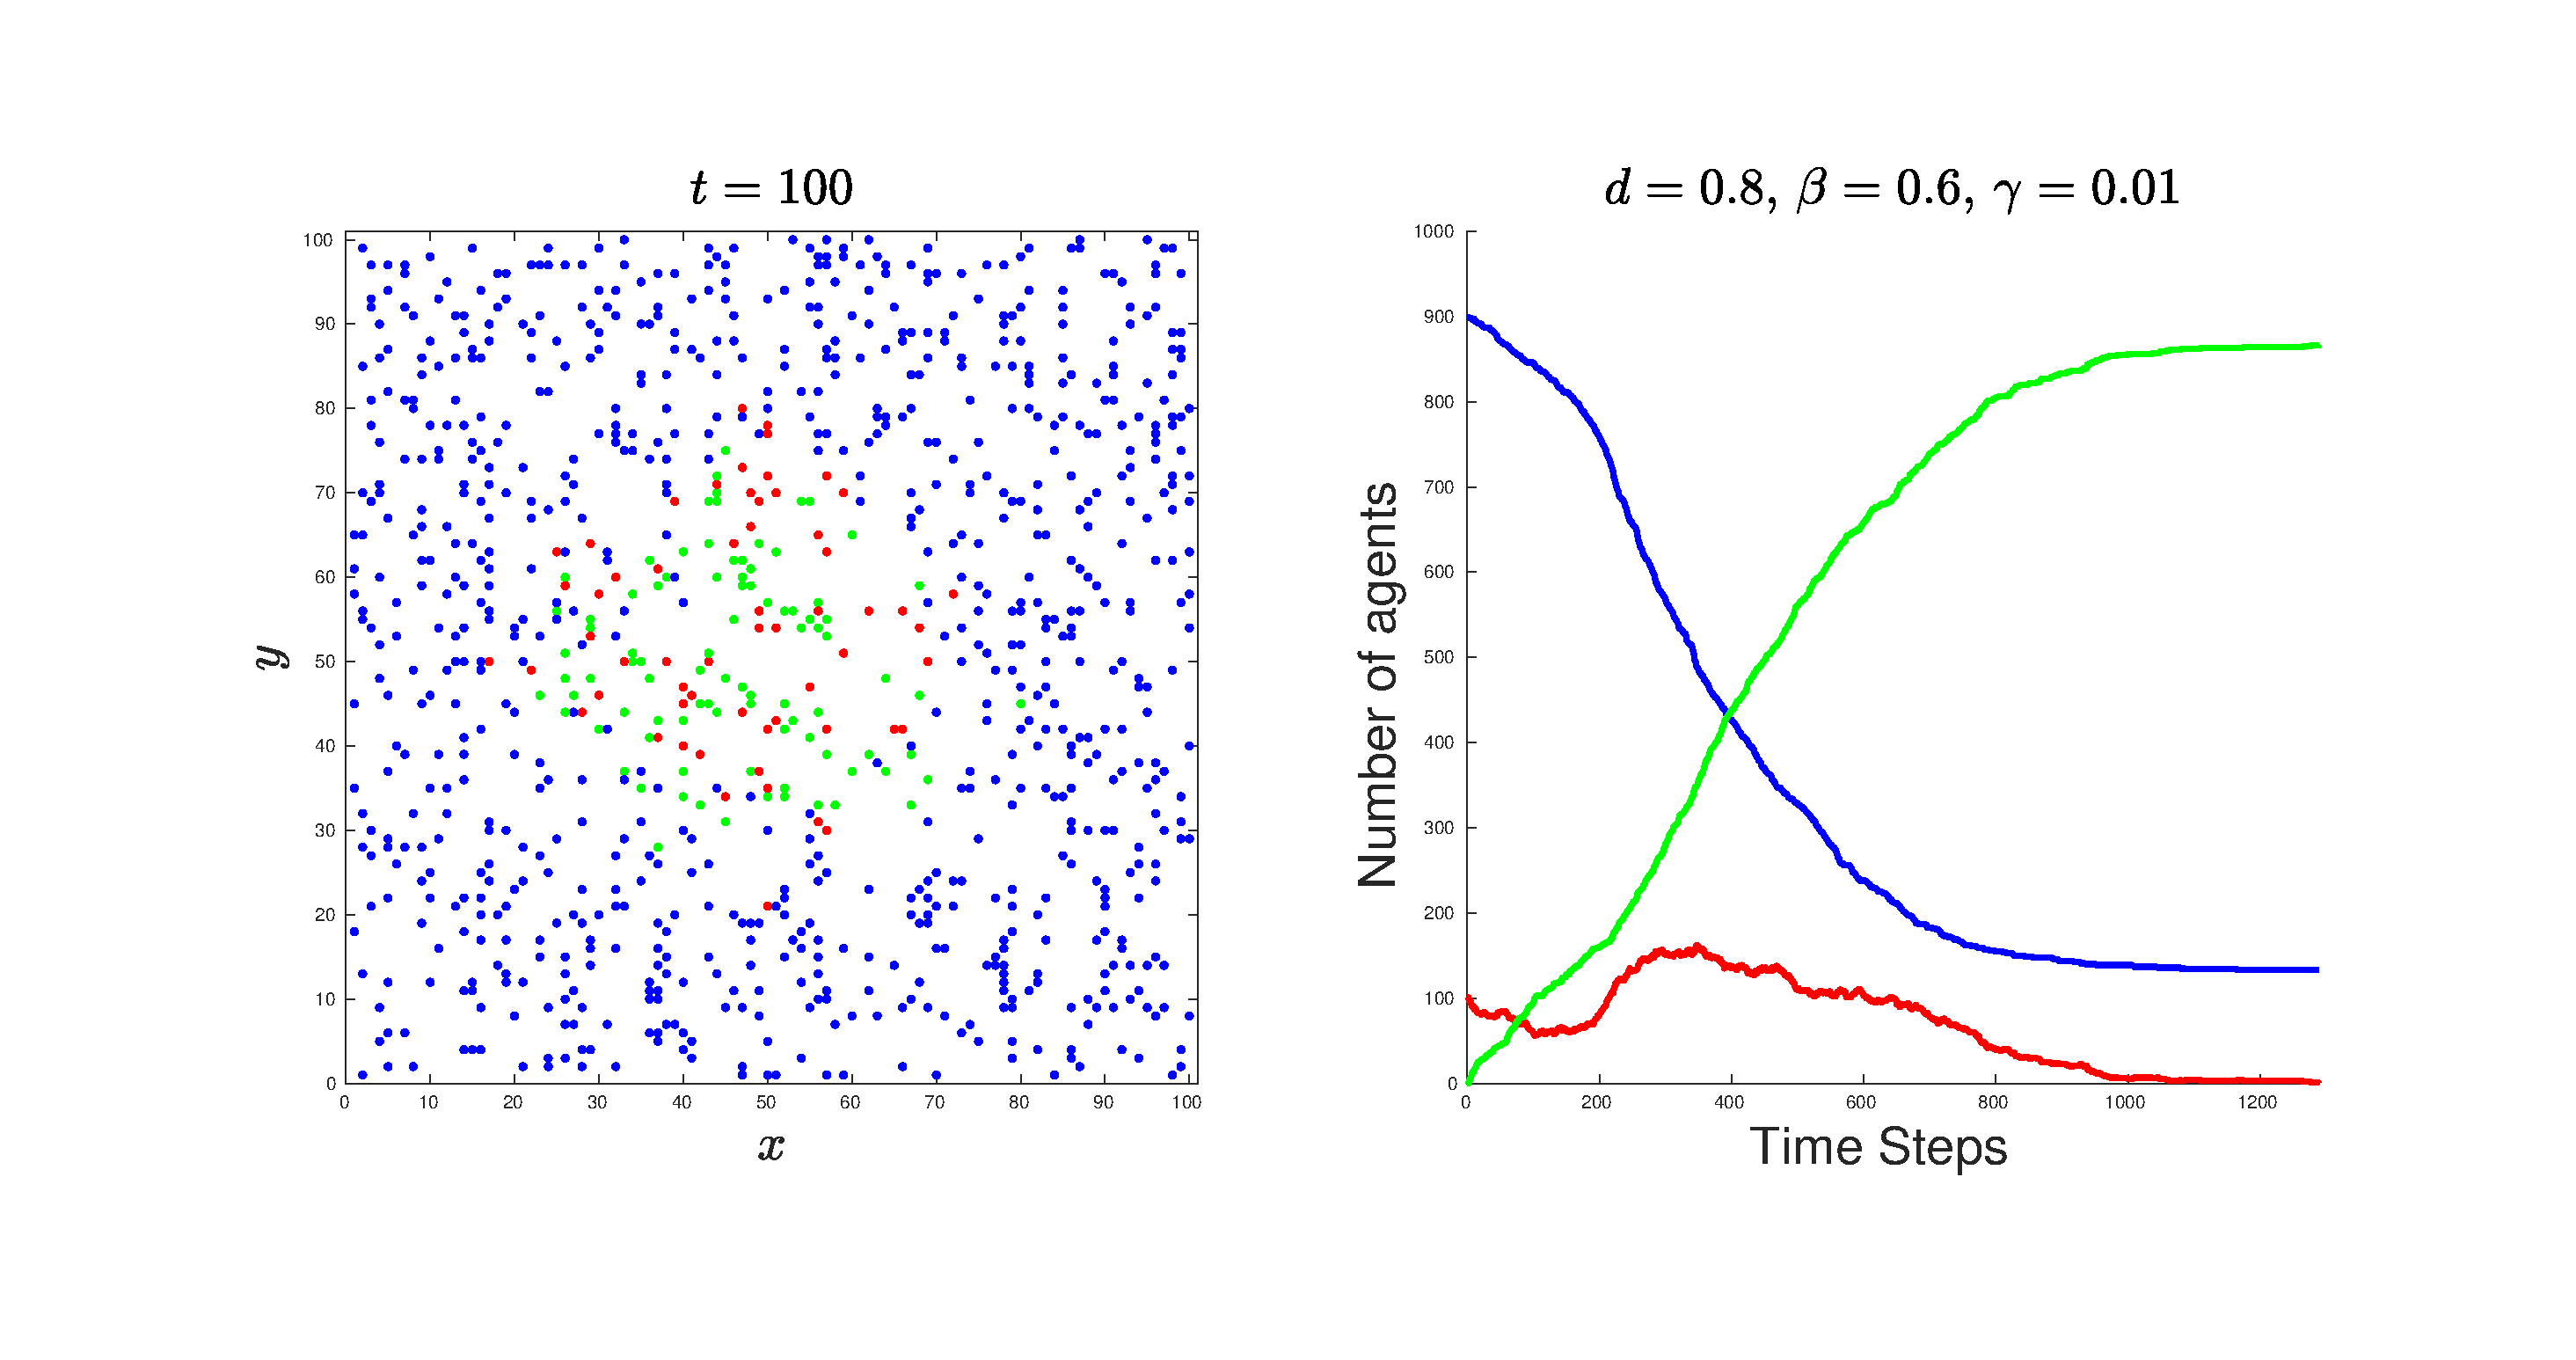
\includegraphics[width=0.9\linewidth]{1_1000_agents}
	\caption{Plot of the proportions of susceptible (blue), infected (red) and recovered (green) individuals in each state over time.}%
	\label{fig:2}
\end{figure}

With the above stated parameters ($d=0.8$, $\beta=0.6$, $\gamma=0.01$), the disease does not spread over the whole population. However more than 80\% were infected over time, which could be a very likely scenario of the corona outbrake.


\subsection{Improving the Simulation}
Random walk is commonly used for simple Simulations. However, this movement pattern does not represent the daily routine of the majority of citizens. It  is more likely that the major part of the population moves around their hometown and travels small distances which leads to clustering of the whole population. To improve the simulation, the agents are split into two groups. One group moves random walk like. This group represents e.g. service providers and delivery services. The other group moves around given points. This movement is implemented using polar coordinates with random radius and random angle. The movement pattern of the two groups is illustrated in Figure \ref{fig:movementPattern}. 
\begin{figure}[H]
	\centering
	\includegraphics[width=0.9\linewidth]{img/movementPattern.png}
	\caption{Movement pattern of the two groups. Random walk (orange) and localized movement (blue).}%
	\label{fig:movementPattern}
\end{figure}

With these two groups, new features such as multiple outbreaks in different clusters can be observed. An example of the improved model is shown in Figure \ref{fig:multipleOutbreaks}. In this case, 3000 agents were initialized on a 200 by 200 grid with the infection parameters $\beta=0.6$ and $\gamma = 0.01$. $70\%$ of the agents move in clusters. The infection waves at $t = 40$, $t = 210$ and $t= 650$ can be explained by the infection of a new cluster. The second infection wave is illustrated in Figure \ref{fig:clusterInfection}. The whole simulation can be found  as a video \url{https://youtu.be/c7ehtN-1n9w}.

\begin{figure}[H]
	\centering
	\includegraphics[width=0.7\linewidth]{img/multipleOutbreaks.pdf}
	\caption{Plot  of  the  proportions  of  susceptible  (blue),  infected  (orange)  and  recovered  (green)  individuals  in  each  state over time.}%
	\label{fig:multipleOutbreaks}
\end{figure}

\begin{figure}[H]
    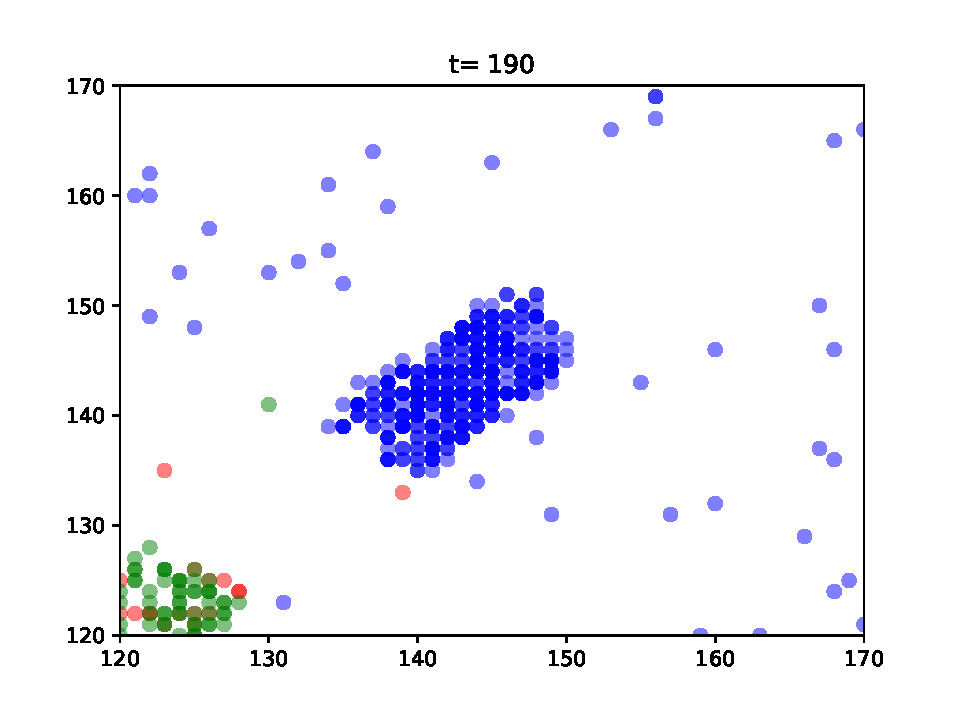
\includegraphics[width=.24\textwidth]{img/cluster190.pdf}\hfill
    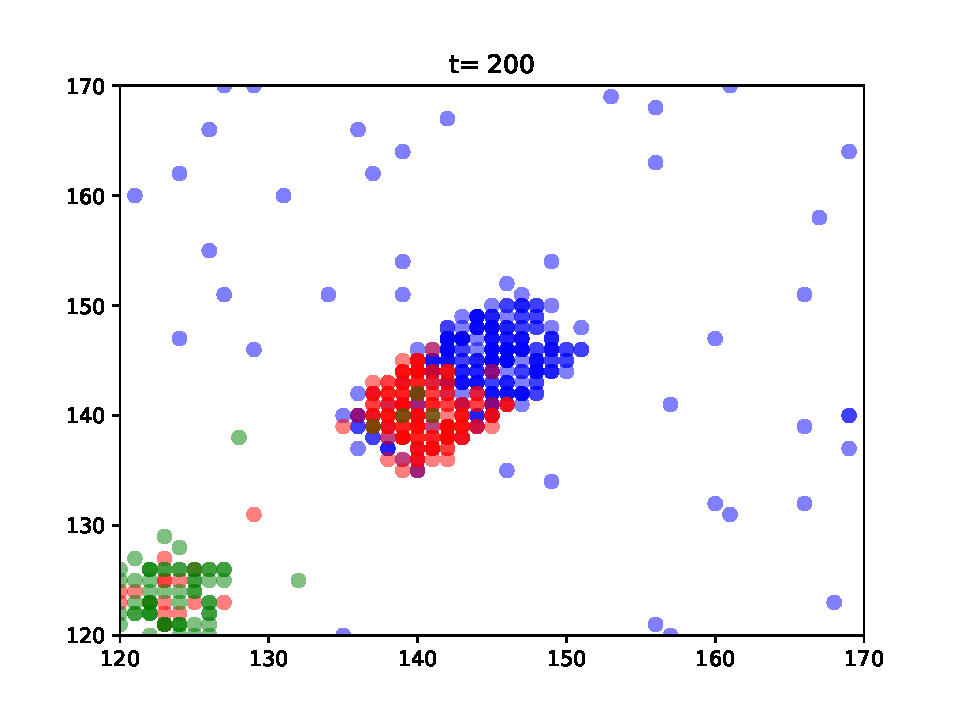
\includegraphics[width=.24\textwidth]{img/cluster200.pdf}\hfill
    \\[\smallskipamount]
    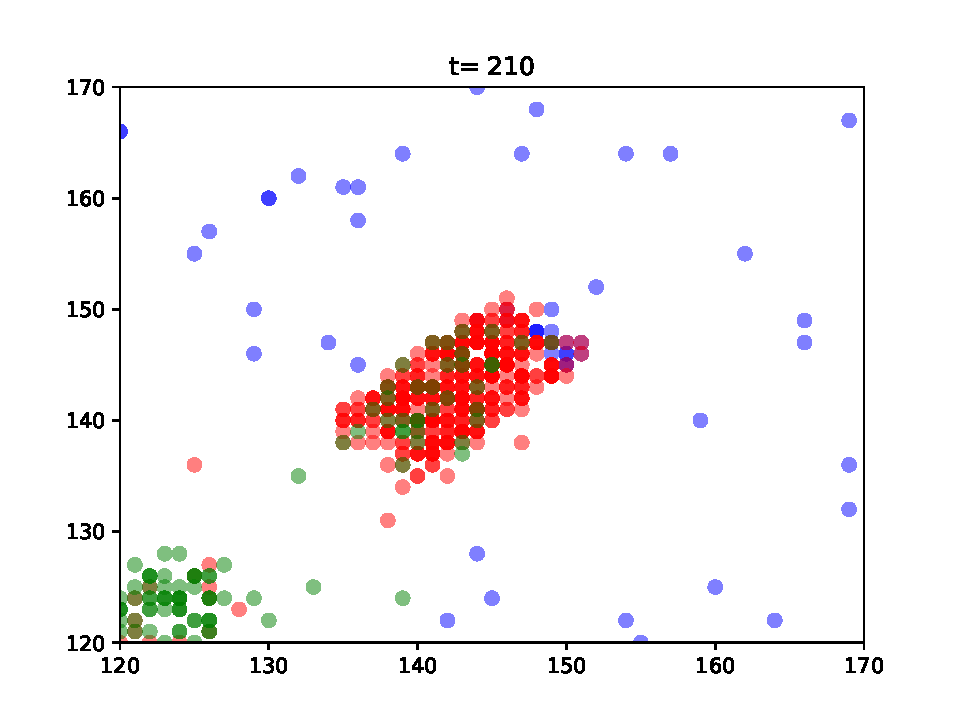
\includegraphics[width=.24\textwidth]{img/cluster210.pdf}\hfill
    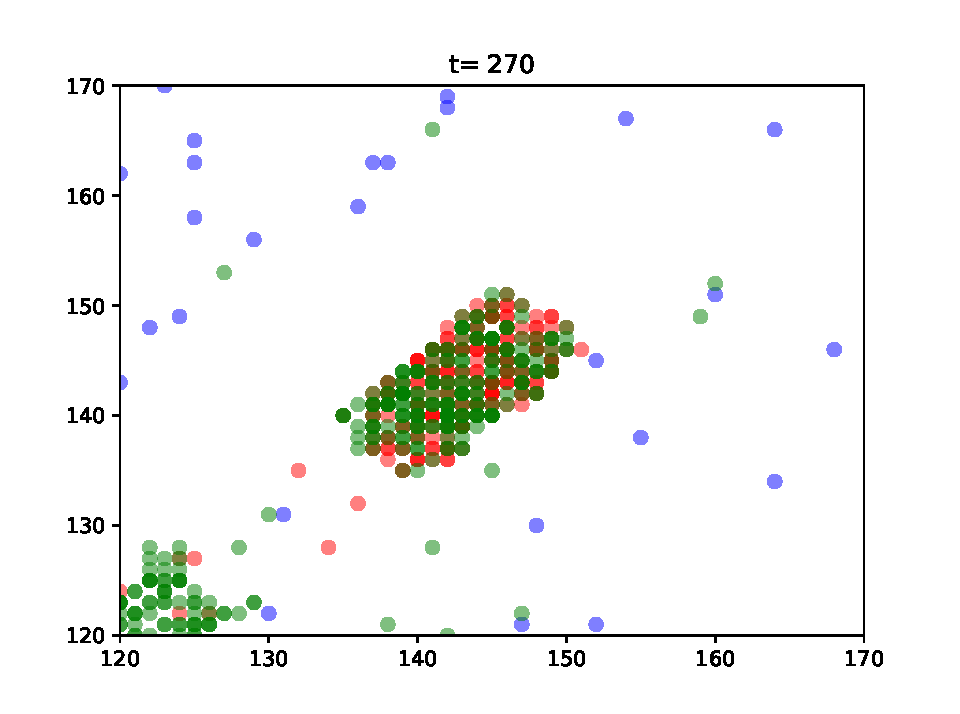
\includegraphics[width=.24\textwidth]{img/cluster270.pdf}\hfill
    \caption{Second infection wave from figure~\ref{fig:multipleOutbreaks}. Blue: susceptibles, red: infected, green: recovered. $t = 190$ cluster gets infected (top left), $t = 200$ disease spreads (top right ), $t = 210$ most of the cluster is infected (bottom left) and $t = 270$ cluster recovers (bottom right).}%
    \label{fig:clusterInfection}
    
\end{figure}

\section{\label{sec:outlook}Outlook}

% !TeX root = ./corona_contact_tracing.tex
% chktex-file 46
% !TeX spellcheck = en-GB
% !TeX encoding = utf8

\section{Outlook}
This section presents future approaches to optimally reduce the spread of the disease with minimal societal intervention.

\subsection{Edge Cutting}
All non pharmaceutical interventions (NPI) could be understood as some kind of edge removal in our graph-based approach:
\begin{itemize}
	\item Isolation of an infected individual removes all of its edges with very high probability.
	\item Quarantine of a contact person removes all of its edges with high probability.
	\item Social distancing removes some edges of of many individuals.
	\item Cancellation of large events remove many edges of many individuals.
\end{itemize}
These interventions can be modelled in our SIR model by modifying the diffusion rate of the agents.
Thus its effects can be evaluate qualitatively and quantitatively.

Based on our graph-based approach, one could also try to compute the minimal set of interventions, which still contains the disease.
A good proxy for this containment is to analyse the effect of these measures on $R_0$, which models how many people are infected by a single infected person.
It is crucial to constrain $R_0$ below one to avoid exponential growth of the number of infected individuals.

In our approach $R_0$ can be derived from the ratio of infected people of $H^{(t+1)}$ and of $H^{(t)}$:
\begin{equation}
	R_0 = \frac{\norm{H^{(t+1)}\mid_{m=1}}_{0}}{\norm{H^{(t)}\mid_{m=1}}_{0}} %#TODO betrag
\end{equation}

The square matrix $C$ with dimensions $N \times N$ models desirable edge cancellations.
Note, that this matrix does not have to know the edges of a future time step, it only expresses which edges must not exist.
It is multiplied element-wise onto the adjacency matrix $A$, thus $\bar{A} = A \odot C$ describes a adjacency matrix with applied cancellations.

To optimally limit the spread of the disease, we seek to minimize the number of cancellations $\norm{C}_0$, given that $R_0$ is below one:
\begin{equation}
	\max_{C} \norm{C}_0\text{, s.t. }R_0 < 1
\end{equation}
Alternatively

\begin{equation}
	\max_{C} \norm{C}_0\text{, s.t. } \norm{H^{(t+1)}\mid_{m=1}}_{0} <= KapaLimit
\end{equation}

% Future Work: This would be more powerful, if there would be some different kinds of edges (social, work, education, large events, etc.)\\
% Future Work: This only takes the current time step into account but it would be desirable to look even further into the future.

\subsection{Test Prioritization}
When tests are limited, they should be used to discover as much as possible about the health state of the overall population.
This in turn allows to reduce the $R_0$ value in further time steps as edge cutting becomes more efficient.

Lets assume there are $t_{\text{max}}$ tests per time step.
A test reveals the true health state of an individual (ignoring false negatives and false positives)
\begin{equation}
	h_{{v}_i}^{(t)} \xrightarrow{\text{test}} h_{{v}_i}^{(t+1)} \in \{\vec{e}_0, \vec{e}_1, \vec{e}_2 \}
\end{equation}

The test assignment $T$ with dimension $N$ is a binary variable describing which individuals should be tested.

\appendix{Appendix}

% !TeX root = ./algorithm_notes.tex
% chktex-file 46
% !TeX spellcheck = en-GB
% !TeX encoding = utf8

\section{Appendix}

\subsection{Consistency of notations}%
\label{sec:consistency}

Using the notation from the blog and the paper, including $H'\in\mathbb{R}^{N\times D}$, $A\in\mathbb{R}^{N\times N}$, $H\in\mathbb{R}^{N\times D}$, the propagation rule is:

\begin{equation}
	H' = A H
\end{equation}

is equivalent to

\begin{equation}
	\begin{split}
		H'_{v_i, m} & = \sum_l \overbrace{A_{v_i, l}}^{\in \{0, 1\}} H_{l, m} \\
		            & = \sum_{l'} H_{l',m}
	\end{split}
\end{equation}

where $l'$ takes all $A_{v_i,l}=1$, i.e.\ neighbours, into account.

Hence, I do understand that the notations are equal.

\subsection{Formulate normalisation}

Use from ICLR 2017 paper the normalisation $D_{ii} = \sum_j \hat{A}_{ij}$.

Use the knowledge from the blog post to write:

\begin{equation}
	\begin{split}
		\overbrace{H'}^{\in \mathbb{R}^{N\times D}} 
			& = \overbrace{D^{-1}}^{\in\mathbb{R}^{N\times N}} \overbrace{\hat{A}}^{\in \mathbb{R}^{N\times N}} \overbrace{H}^{\in\mathbb{R}^{N\times D}}
			\Leftrightarrow H'_{v_i, m} = \sum_k \overbrace{D^{-1}_{v_i,k}}^{=D_{v_i,v_i}, \delta_{v_i, k}} {(\hat{A} H)}_{km} \\
			& = D^{-1}_{v_i, v_i} (\hat{A} H)_{v_i, m} = D^{-1}_{{v}_i, v_i} \sum_k \hat{A}_{v_i, k} H_{k, m} = \sum_k \underbrace{\frac{\hat{A}_{v_i, k}}{\sum_j \hat{A}_{v_i, j}}}_{\text{normalised}} H_{k, m}.
	\end{split}
\end{equation}

The weighting by the adjacency matrix is, indeed, normalised to its column sums.

Note that this part is also normalised:

\begin{equation}
\begin{split}
	\sum_m H'_{v_i, m} & = \sum_m \sum_k \frac{\hat{A}_{v_i, k}}{\sum_j \hat{A}_{v_i, j}} H_{k, m} \\
	& = \sum_k \frac{\hat{A}_{v_i, k}}{\sum_j \hat{A}_{v_i, j}} \underbrace{\sum_m H_{k,m}}_{=1\text{, per construction}} = 1
\end{split}
\end{equation}

\end{document}
%
% ****** End of file apssamp.tex ******
